% Provenance (never printed): cycle 2 "Questionner l'espace et le temps ---
% se situer dans l'espace": representations of familiar spaces (plans), "lire
% des plans, se reperer sur des cartes. Elements constitutifs d'une carte :
% titre, echelle, orientation, legende"; see sources/book1/PROVENANCE.md.
% Book 1, grade 2, chapter 2. Sync 1: "scale" is owned here; "cardinal
% directions" is the physics series' term (prose only); "compass rose" here.
\chapter{From a Drawing to a Map}\label{ch:g2:drawing-to-map}

A pigeon flies over the school. What does it see? Not the front doors, not
the windows, not the children's faces: from up there it sees only the tops
of things. The roofs of the buildings are grey rectangles. The yard is a
big empty shape with a few round treetops. The paths are thin lines. The
pigeon sees the school from above --- the way a \omterm{def:g2:drawing-to-map:map}{map} shows it.

\begin{omfigure}
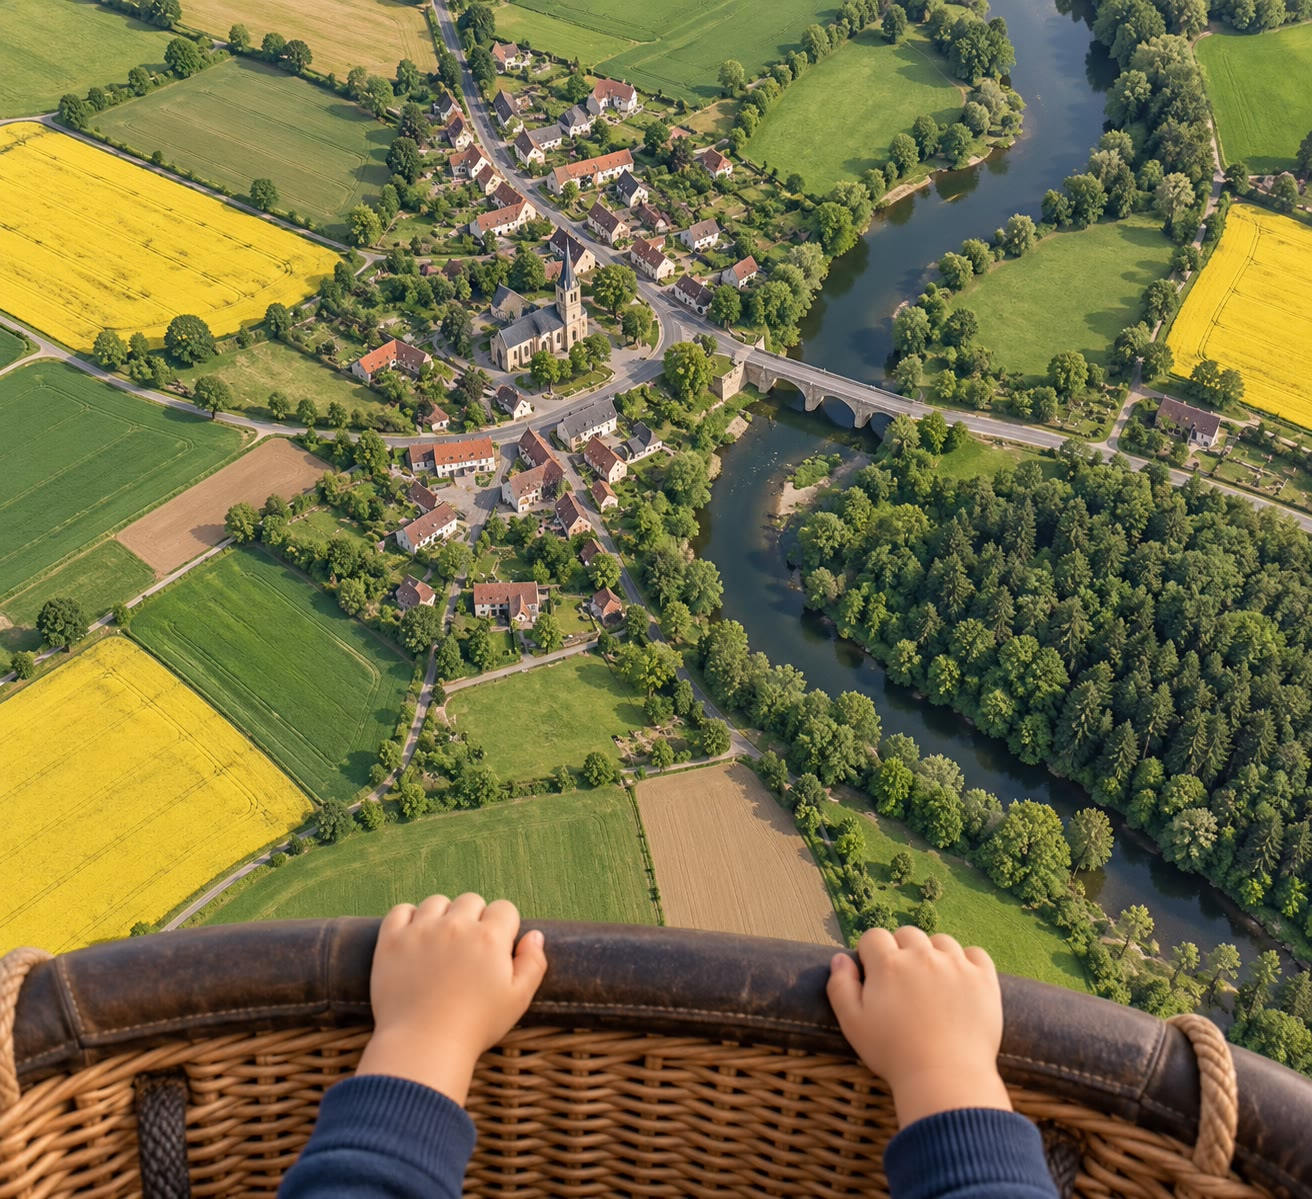
\includegraphics[width=0.62\linewidth]{images/book1/ai/g2-balloon-view.jpg}

{\small The countryside seen from a hot-air balloon: fields, a village, a
road, a \omterm{def:g1:landscapes-around-us:water}{river} and its bridge, all seen from above.}
\end{omfigure}

\section{Seen from the side, seen from above}

Put a few toy blocks on a table. Look at them from the side: you see their
height, and the ones at the back are hidden behind the ones in front. Now
stand up and look down on them from above: you no longer see how tall they
are, but you see exactly where each one is, and how far apart they are.

\begin{omfigure}
\begin{tikzpicture}[x=1cm, y=1cm, font=\small]
  % side view
  \begin{scope}
    \draw[black!50] (-0.2,0) -- (4.6,0);
    \fill[red!55, draw=black!60] (0.2,0) rectangle (1.2,1.6);
    \fill[ocBlue!55, draw=black!60] (1.6,0) rectangle (3.0,0.8);
    \fill[yellow!70, draw=black!60] (3.4,0) -- (3.9,1.1) -- (4.4,0) -- cycle;
    \node at (2.2,-0.5) {seen from the side};
  \end{scope}
  % from above
  \begin{scope}[shift={(6.4,0)}]
    \draw[black!30, fill=black!3] (-0.2,-0.1) rectangle (4.6,2.3);
    \fill[red!55, draw=black!60] (0.2,0.4) rectangle (1.2,1.4);
    \fill[ocBlue!55, draw=black!60] (1.6,1.0) rectangle (3.0,2.0);
    \fill[yellow!70, draw=black!60] (3.9,0.75) circle (0.5);
    \node at (2.2,-0.5) {seen from above};
  \end{scope}
\end{tikzpicture}

{\small Three blocks on a table: a tall red block, a flat blue block and a
yellow cone. From above, the cone is a circle and the tall block is a
square.}
\label{fig:g2:drawing-to-map:blocks}
\end{omfigure}

\begin{definition}[Plan]\label{def:g2:drawing-to-map:plan}
A \emph{plan}\index{plan} is a drawing of a small place --- a room, a
house, a school, a garden --- as it is seen from straight above, drawn
smaller than it really is but with every part in its right place.
\end{definition}

\section{Drawing smaller: the scale}

A classroom is far too big to draw on a sheet of paper as it is. We draw it
smaller --- but every part must be smaller in the same way, or the \omterm{def:g2:drawing-to-map:plan}{plan}
will lie. The easiest way is to use squared paper: one square of the paper
stands for one metre of the classroom.

\begin{definition}[Scale]\label{def:g2:drawing-to-map:scale}
The \emph{scale}\index{scale} of a \omterm{def:g2:drawing-to-map:plan}{plan} or a \omterm{def:g2:drawing-to-map:map}{map} tells how much smaller the
drawing is than the real place: how far on the ground a length on the
drawing stands for. For example: \emph{1 square stands for 1 metre}.
\end{definition}

\begin{omfigure}
\begin{tikzpicture}[x=0.75cm, y=0.75cm, font=\scriptsize]
  \draw[black!15] (0,0) grid (10,8);
  \draw[black, line width=1.6pt] (0,0) rectangle (10,8);
  % board on the north wall
  \fill[black!70] (3,7.8) rectangle (7,8);
  % teacher's desk
  \fill[brown!50, draw=black!70] (4,6) rectangle (6,7);
  % pupils' desks: 3 rows of 3
  \foreach \x in {1,4,7} \foreach \y in {1,2.5,4}
    \fill[orange!45, draw=black!70] (\x,\y) rectangle ++(2,1);
  % cupboard
  \fill[ocBlue!40, draw=black!70] (9,5) rectangle (10,8);
  % door (gap) on the east wall, windows on the west wall
  \fill[white] (9.85,1) rectangle (10.15,2);
  \draw[black!70] (10,2) arc[start angle=90, end angle=180, radius=1];
  \foreach \y in {1.5,4.5}
    \draw[ocBlue, line width=2.5pt] (0,\y) -- (0,\y+2);
  % legend
  \begin{scope}[shift={(11,7.2)}]
    \node[anchor=west, font=\small\bfseries] at (0,0.4) {The classroom};
    \fill[black!70] (0,-0.25) rectangle (0.8,-0.05); \node[anchor=west] at (1,-0.15) {board};
    \fill[brown!50, draw=black!70] (0,-1.1) rectangle (0.8,-0.7); \node[anchor=west] at (1,-0.9) {teacher's desk};
    \fill[orange!45, draw=black!70] (0,-1.85) rectangle (0.8,-1.45); \node[anchor=west] at (1,-1.65) {pupils' desk};
    \fill[ocBlue!40, draw=black!70] (0,-2.6) rectangle (0.8,-2.2); \node[anchor=west] at (1,-2.4) {cupboard};
    \draw[ocBlue, line width=2.5pt] (0,-3.15) -- (0.8,-3.15); \node[anchor=west] at (1,-3.15) {window};
    \draw[black!70] (0.8,-3.95) arc[start angle=0, end angle=90, radius=0.6]; \draw[black, line width=1.6pt] (0.2,-3.95) -- (0.8,-3.95); \node[anchor=west] at (1,-3.7) {door};
    \draw[black!15] (0,-4.9) rectangle (0.75,-4.15);
    \node[anchor=west] at (1,-4.53) {1 square = 1 metre};
    \pic[scale=0.7, transform shape] at (0.7,-6.2) {compassrose};
  \end{scope}
\end{tikzpicture}

{\small The \omterm{def:g2:drawing-to-map:plan}{plan} of a classroom on squared paper, with its title, its
\omterm{def:g2:drawing-to-map:legend}{legend}, its \omterm{def:g2:drawing-to-map:scale}{scale} and its \omterm{def:g2:drawing-to-map:directions}{compass rose}. The north wall, with the board, is
at the top.}
\label{fig:g2:drawing-to-map:classroom}
\end{omfigure}
% (exercise data: an invented classroom of 10 m by 8 m)

\begin{method}[Measuring on a plan]\label{met:g2:drawing-to-map:measure}
To find a real length on a \omterm{def:g2:drawing-to-map:plan}{plan} drawn on squares:
\begin{enumerate}
  \item count the squares along the length you want;
  \item read the \omterm{def:g2:drawing-to-map:scale}{scale}: how much one square stands for;
  \item give the answer in metres (or in kilometres on a \omterm{def:g2:drawing-to-map:map}{map}).
\end{enumerate}
\end{method}

\begin{example}[How long is the classroom?]\label{ex:g2:drawing-to-map:length}
Along the north wall of the \omterm{def:g2:drawing-to-map:plan}{plan} there are 10 squares. One square stands
for 1 metre, so the classroom is 10 metres long. Along the west wall there
are 8 squares: it is 8 metres wide. The board covers 4 squares of the north
wall: it is 4 metres long.
\end{example}

\begin{omfigure}
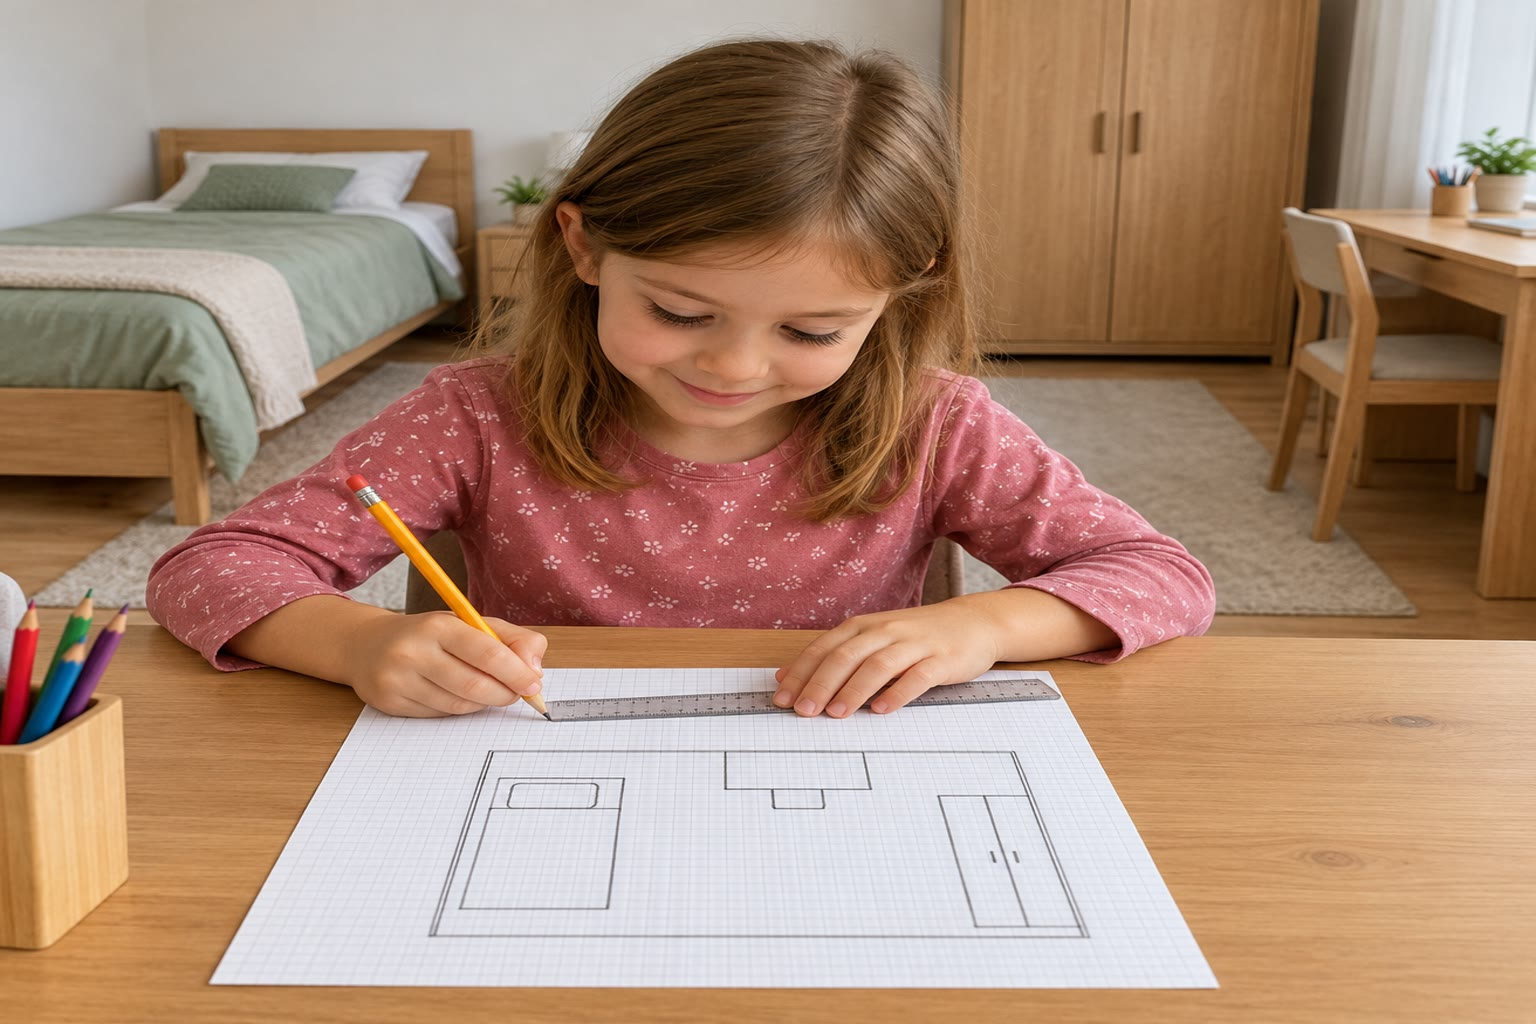
\includegraphics[width=0.55\linewidth]{images/book1/ai/g2-bedroom-plan.jpg}

{\small Drawing the \omterm{def:g2:drawing-to-map:plan}{plan} of a bedroom on squared paper.}
\end{omfigure}

\section{From a plan to a map}

A \omterm{def:g2:drawing-to-map:plan}{plan} shows a small place. When we draw a bigger place --- a whole town, a
\omterm{def:g1:landscapes-around-us:landform}{valley}, a country --- we draw a \omterm{def:g2:drawing-to-map:map}{map}.

\begin{definition}[Map]\label{def:g2:drawing-to-map:map}
A \emph{map}\index{map} is a drawing of a large part of the Earth's
surface, seen from above and drawn much smaller than it really is.
\end{definition}

On a \omterm{def:g2:drawing-to-map:map}{map}, a house is far too small to draw as it really is, so \omterm{def:g2:drawing-to-map:map}{map} makers
use small signs: a dot for a farm, a blue line for a \omterm{def:g1:landscapes-around-us:water}{river}, a green shape
for a wood. The meaning of every sign is given in a box beside the \omterm{def:g2:drawing-to-map:map}{map}.

\begin{definition}[Legend]\label{def:g2:drawing-to-map:legend}
A \emph{map symbol}\index{map symbol} is a small sign that stands for one
kind of thing on a \omterm{def:g2:drawing-to-map:plan}{plan} or a \omterm{def:g2:drawing-to-map:map}{map}. The \emph{legend}\index{legend} is the box
that shows every symbol of the \omterm{def:g2:drawing-to-map:map}{map} with its meaning.
\end{definition}

\section{Finding our way: the four directions and the compass rose}

To say where something is, ``on the left'' or ``on the right'' is not
enough: what is on your left is on the right of someone facing you. People
use four directions that are the same for everybody: north, east, south and
west. You have met them in the physics books, with the compass. In the
morning the Sun rises in the east, and in the evening it sets in the west;
north and south are halfway between them, opposite each other.

\begin{omfigure}
\begin{tikzpicture}[font=\small]
  \pic[scale=1.5, transform shape] at (0,0) {compassrose};
  \node[align=left, anchor=west, font=\small] at (2.6,0.3)
    {N = north (at the top of most maps)\\E = east (on the right)\\S = south (at the bottom)\\W = west (on the left)};
\end{tikzpicture}

{\small A \omterm{def:g2:drawing-to-map:directions}{compass rose}. Between north and east is north-east; between
south and west, south-west.}
\label{fig:g2:drawing-to-map:rose}
\end{omfigure}

\begin{definition}[Compass rose]\label{def:g2:drawing-to-map:directions}
A \emph{compass rose}\index{compass rose} is the star drawn on a \omterm{def:g2:drawing-to-map:map}{map} that
shows the directions north, east, south and west. On most \omterm{def:g2:drawing-to-map:map}{maps} north is at
the top, east on the right, south at the bottom and west on the left.
\end{definition}

\begin{safety}
Never look at the Sun to find east or west: it can hurt your eyes for ever.
Look at the shadows instead, or use a compass.
\end{safety}

\section{Reading a real map}

Every good \omterm{def:g2:drawing-to-map:map}{map} has four parts: a \textbf{title} that says what the \omterm{def:g2:drawing-to-map:map}{map}
shows, a \textbf{\omterm{def:g2:drawing-to-map:legend}{legend}}, a \textbf{\omterm{def:g2:drawing-to-map:scale}{scale}}, and a \textbf{\omterm{def:g2:drawing-to-map:directions}{compass rose}}
(or at least an arrow pointing north). Here is the \omterm{def:g2:drawing-to-map:map}{map} of a hilly \omterm{def:g1:landscapes-around-us:landform}{valley},
the Varden Hills. It is the invented \omterm{def:g1:landscapes-around-us:landform}{valley} that you will meet again and
again in this book and in the next ones, each time drawn in more detail.

\begin{omfigure}
\begin{tikzpicture}
\begin{axis}[width=9.6cm, scale only axis,
    xmin=0, xmax=10, ymin=0, ymax=8, axis equal image,
    xtick={0,...,10}, ytick={0,...,8}, xticklabels={}, yticklabels={},
    grid=major, grid style={black!20}, major tick length=0pt,
    axis background/.style={fill=green!12!omLithAlluv},
    title={\textbf{The Varden Hills}}]
  \addplot[fill=omHypsLandD, draw=omHypsLandE!80!black, line width=0.4pt, fill opacity=0.85,
    unbounded coords=jump, even odd rule] table {figdata/out/grade-2-varden_plan-hills.dat};
  \addplot[fill=green!45!black!55, draw=green!35!black, line width=0.4pt] table {figdata/out/grade-2-varden_plan-wood.dat};
  \addplot[ocBlue!85!black, line width=2.2pt] table {figdata/out/shared-region-river.dat};
  \addplot[red!65!black, line width=1.3pt] table {figdata/out/grade-2-varden_plan-road.dat};
  \fill[black] (axis cs:5.012,3.414) ++(-3pt,-4pt) rectangle ++(6pt,8pt);
  \fill[white] (axis cs:5.012,3.414) ++(-1.6pt,-4pt) rectangle ++(3.2pt,8pt);
  \fill[brown!70!black] (axis cs:2.5,3.5) ++(-3.5pt,-3.5pt) rectangle ++(7pt,7pt);
  \fill[red!70!black] (axis cs:7.5,5.5) ++(-5pt,-3pt) rectangle ++(4pt,4pt);
  \fill[red!70!black] (axis cs:7.5,5.5) ++(1pt,-3pt) rectangle ++(4pt,4pt);
  \fill[red!70!black] (axis cs:7.5,5.5) ++(-2pt,2pt) rectangle ++(4pt,4pt);
\end{axis}
\begin{scope}[shift={(10.2,6.4)}, font=\small]
  \node[anchor=west, font=\small\bfseries] at (-0.1,0.55) {Legend};
  \fill[omHypsLandD, draw=omHypsLandE!80!black] (0,-0.2) rectangle (0.7,0.15); \node[anchor=west] at (0.85,0) {hills};
  \fill[green!45!black!55] (0,-0.85) rectangle (0.7,-0.5); \node[anchor=west] at (0.85,-0.67) {wood};
  \draw[ocBlue!85!black, line width=2.2pt] (0,-1.35) -- (0.7,-1.35); \node[anchor=west] at (0.85,-1.35) {river};
  \draw[red!65!black, line width=1.3pt] (0,-2.0) -- (0.7,-2.0); \node[anchor=west] at (0.85,-2.0) {road};
  \fill[black] (0.25,-2.8) rectangle (0.45,-2.5); \fill[white] (0.3,-2.8) rectangle (0.4,-2.5); \node[anchor=west] at (0.85,-2.65) {bridge};
  \fill[brown!70!black] (0.23,-3.45) rectangle (0.47,-3.21); \node[anchor=west] at (0.85,-3.33) {farm};
  \foreach \dx/\dy in {0.12/-4.1, 0.33/-4.1, 0.22/-3.92}
    \fill[red!70!black] (\dx,\dy) rectangle ++(0.13,0.13);
  \node[anchor=west] at (0.85,-3.98) {village};
  \draw[black!40] (0,-4.95) rectangle (0.5,-4.45); \node[anchor=west, align=left] at (0.85,-4.7) {1 square\\= 1 kilometre};
  \pic[scale=0.75, transform shape] at (0.8,-6.5) {compassrose};
\end{scope}
\end{tikzpicture}

{\small A simple \omterm{def:g2:drawing-to-map:map}{map} of the Varden Hills, with its title, its \omterm{def:g2:drawing-to-map:legend}{legend}, its
\omterm{def:g2:drawing-to-map:scale}{scale} and its \omterm{def:g2:drawing-to-map:directions}{compass rose}. The \omterm{def:g1:landscapes-around-us:water}{river} flows from west to east.}
\label{fig:g2:drawing-to-map:varden}
\end{omfigure}
% (figdata/grade-2/varden_plan.py; the region: figdata/shared/region.py)

\begin{method}[Reading a map]\label{met:g2:drawing-to-map:read}
\begin{enumerate}
  \item Read the title: what place does the \omterm{def:g2:drawing-to-map:map}{map} show?
  \item Read the \omterm{def:g2:drawing-to-map:legend}{legend}: what does each symbol mean?
  \item Find the \omterm{def:g2:drawing-to-map:directions}{compass rose}: where is north?
  \item Read the \omterm{def:g2:drawing-to-map:scale}{scale}, and count squares to find distances.
\end{enumerate}
\end{method}

\begin{example}[From the farm to the village]\label{ex:g2:drawing-to-map:farm}
On the \omterm{def:g2:drawing-to-map:map}{map} of the Varden Hills, the farm is south of the \omterm{def:g1:landscapes-around-us:water}{river}. To go to
the village, the farmer takes the road eastwards, crosses the \omterm{def:g1:landscapes-around-us:water}{river} on the
bridge, and goes on to the north-east. The village is 5 squares east of the
farm and 2 squares north of it: that is 5 kilometres to the east and 2
kilometres to the north.
\end{example}

\section{Exercises}

\begin{exercise}[$\star$]\label{exo:g2:drawing-to-map:1}
Is a \omterm{def:g2:drawing-to-map:plan}{plan} drawn as seen from the side, or as seen from above?
\end{exercise}

\begin{exercise}[$\star$]\label{exo:g2:drawing-to-map:2}
On the \omterm{def:g2:drawing-to-map:plan}{plan} of the classroom, what is drawn in blue on the west wall? What
is in the north-east corner?
\end{exercise}

\begin{exercise}[$\star$]\label{exo:g2:drawing-to-map:3}
Name the four parts that every good \omterm{def:g2:drawing-to-map:map}{map} should have.
\end{exercise}

\begin{exercise}[$\star$]\label{exo:g2:drawing-to-map:4}
On most \omterm{def:g2:drawing-to-map:map}{maps}, which direction is at the top? Which is on the left?
\end{exercise}

\begin{exercise}[$\star$]\label{exo:g2:drawing-to-map:5}
On the \omterm{def:g2:drawing-to-map:plan}{plan} of the classroom, a pupils' desk covers 2 squares by 1 square.
How long and how wide is a desk in the real classroom?
\end{exercise}

\begin{exercise}[$\star$]\label{exo:g2:drawing-to-map:6}
On the \omterm{def:g2:drawing-to-map:map}{map} of the Varden Hills, what does the brown square stand for? And
the green shape?
\end{exercise}

\begin{exercise}[$\star\star$]\label{exo:g2:drawing-to-map:7}
On the \omterm{def:g2:drawing-to-map:map}{map} of the Varden Hills, is the wood north or south of the \omterm{def:g1:landscapes-around-us:water}{river}?
Is it east or west of the farm?
\end{exercise}

\begin{exercise}[$\star\star$]\label{exo:g2:drawing-to-map:8}
On the \omterm{def:g2:drawing-to-map:map}{map} of the Varden Hills, the whole \omterm{def:g2:drawing-to-map:map}{map} is 10 squares from west to
east and 8 squares from south to north. How many kilometres is that in each
direction?
\end{exercise}

\begin{exercise}[$\star\star$]\label{exo:g2:drawing-to-map:9}
On the classroom \omterm{def:g2:drawing-to-map:plan}{plan}, how many pupils' desks are there? A pupil sits at
the desk nearest to the door. Is it in the north or in the south of the
classroom?
\end{exercise}

\begin{exercise}[$\star\star$]\label{exo:g2:drawing-to-map:10}
Lucas draws a \omterm{def:g2:drawing-to-map:plan}{plan} of his bedroom. His bed is 2 metres long. With the \omterm{def:g2:drawing-to-map:scale}{scale}
``1 square stands for 1 metre'', how many squares long is the bed on his
\omterm{def:g2:drawing-to-map:plan}{plan}? His bedroom is 4 metres long and 3 metres wide: how many squares does
the whole room cover?
\end{exercise}

\begin{exercise}[$\star\star$]\label{exo:g2:drawing-to-map:11}
Lena says: ``The \omterm{def:g1:landscapes-around-us:water}{river} is on my left.'' Why does this not tell us where the
\omterm{def:g1:landscapes-around-us:water}{river} is? Say it again in a way that is true for everybody, if she stands on
the farm of the Varden Hills.
\end{exercise}
